\documentclass[a4paper,12pt]{article}
\usepackage[utf8]{inputenc}
\usepackage[cm,empty]{fullpage}
\usepackage[T2A]{fontenc}
\usepackage[english, russian]{babel}
\usepackage{amssymb,amsmath,amsxtra,amsthm}
\usepackage{proof}
\usepackage[pdftex]{graphicx}
\usepackage{wrapfig}
\usepackage{braket}
\usepackage{xcolor}

\usepackage[left=2cm,right=2cm,
    top=1cm,bottom=1cm,bindingoffset=0cm]{geometry}

\renewcommand{\leq}{\leqslant}
\renewcommand{\geq}{\geqslant}


\newcommand{\iiff}{\Longleftrightarrow}
\renewcommand{\iff}{\Leftrightarrow}
\newcommand{\nothing}{\varnothing}

\newtheorem*{rem}{Замечание}

\newcommand{\NN}{\mathbb{N}}
\newcommand{\ZZ}{\mathbb{Z}}
\newcommand{\Q}{\mathbb{Q}}
\newcommand{\A}{\mathbb{A}}
\newcommand{\R}{\mathbb{R}}
\renewcommand{\C}{\mathbb{C}}

\renewcommand{\phi}{\varphi}
\newcommand{\eps}{\varepsilon}

\newcounter{z}


\newcommand{\zs}{\refstepcounter{z}\vskip 10pt\par\noindent
\fbox{\textbf{12.\arabic{z}}} }

\newcommand{\z}{\refstepcounter{z}\vskip 20pt\noindent
\fbox{\textbf{\arabic{z}}} }

\renewcommand{\date}{{\bf 7 марта 2021}} 

\newcommand{\dif}
{
------------------------------------------------------------------------------------------------------------------------------------------------------
}

\newcommand{\HSEhat}{
\vspace*{-0pt}
\noindent
\setcounter{z}{0}


{\bf \phantom{\date}  \large \hfill Математический анализ: \hfill \normalsize \date}

\vspace{5 pt}
{\bf \large \hfill  лекция 3\hfill }

\vspace{15 pt}
\centerline{ \large  Домашнее задание.}
\centerline{ \large  Кирилл Сетдеков}



\vspace*{10pt}
\setcounter{z}{0}

}

\begin{document}
\HSEhat


\subsection*{Задачи}

\begin{enumerate}

\item Найдите $\frac{\partial f}{\partial x} (a,1)$

$$f(x,y) =x + (y-1)\arcsin{\sqrt{\frac{x}{y}}}$$

\textbf{Решение:}\\
Дифференцируем как сумму:

$$\frac{\partial }{\partial x} (x + (y-1)\arcsin{\sqrt{\frac{x}{y}}}) = \frac{\partial }{\partial x} (x) +(y-1)(\frac{\partial }{\partial x} (\arcsin{\sqrt{\frac{x}{y}}})) = 1 + (y-1)(\frac{\partial }{\partial x} (\arcsin{\sqrt{\frac{x}{y}}})) = $$

Применяем цепное правило, где :
$\frac{\partial }{\partial x} (\arcsin{\sqrt{\frac{x}{y}}}) = \frac{\partial \arcsin{u}}{\partial u} \frac{\partial u}{\partial x}$ где $u = \sqrt{\frac{x}{y}} ;\frac{\partial \arcsin{u}}{\partial u} = \frac{1}{\sqrt{1-u^2}}$

$$=1 + (y-1)\frac{\frac{\partial }{\partial x}({\sqrt{\frac{x}{y}}}))}{\sqrt{1-\frac{x}{y}}} =$$

Применяем цепное правило для корня из частного:
$\frac{\partial }{\partial x}({\sqrt{\frac{x}{y}}})) = \frac{\partial \sqrt{u}}{\partial u} \frac{\partial u}{\partial x} $ где $u = \frac{x}{y}; \frac{\partial}{\partial u} (\sqrt{u}) = \frac{1}{2\sqrt{u}}$

и после этого - выносим константу и считаем производную

$$=1 +\frac{\frac{\partial }{\partial x}({{\frac{x}{y}}})}{2\sqrt{\frac{x}{y}}} \frac{y-1}{\sqrt{1-\frac{x}{y}}} =1 +\frac{1}{2y\sqrt{\frac{x}{y}}} \frac{y-1}{\sqrt{1-\frac{x}{y}}} = 1 + \frac{y-1}{2y\sqrt{\frac{x(y-x)}{y^2}}}=1 + \frac{y-1}{2\sqrt{x(y-x)}}$$

Подставим $x = a, y = 1$
$$1 + \frac{1-1}{2\sqrt{a(1-a)}} =1$$


\textbf{Ответ: $1$}


\item Найти градиент и матрицу Гессе
\begin{enumerate}
\item 
$
u = ln(x+y^2)
$

\textbf{Решение:}\\
Градиент по определению - ${grad}_au = (\frac{\partial u}{\partial x}(a), \frac{\partial u}{\partial y}(a))$

Матрица Гессе - квадратная матрица из производных второго порядка по x и y

$$H_a(u) = \begin{pmatrix}
\frac{\partial^2 u}{\partial x^2}(a) & \frac{\partial^2 u}{\partial x \partial y}(a)  \\
\frac{\partial^2 u}{\partial y \partial x}(a) & \frac{\partial^2 u}{\partial y^2}(a) 
\end{pmatrix}$$

Всего надо посчитать 6 производных, начнем с первой производной по х $$\frac{\partial ln(x+y^2)}{\partial x}$$

Используем цепное правило:
$\frac{\partial ln(x+y^2)}{\partial x} = \frac{\partial \ln{u}}{\partial u}\frac{\partial u}{\partial x}$ где $u = x + y^2, \frac{\partial}{\partial u} \ln{u} = \frac{1}{u}$

$$
= \frac{\frac{\partial}{\partial x}(x+y^2)}{x+y^2} = \frac{1}{x+y^2}
$$

Используя ту же замену, считаем: $$\frac{\partial ln(x+y^2)}{\partial y}=\frac{\frac{\partial}{\partial y}(x+y^2)}{x+y^2} = \frac{2y}{x+y^2}$$

Теперь найдем вторые производные.
$$\frac{\partial^2 u}{\partial x^2}(a) = \frac{\partial}{\partial x}(\frac{1}{(x + y^2})=$$

Сделаем замену и используем цепное правило:
где $u = x + y^2; \frac{\partial}{\partial x}(\frac{1}{u})= -\frac{1}{u^2}$

$$=-\frac{ \frac{\partial}{\partial x}(x+y^2)}{(x + y^2)^2} = -\frac{1}{(x + y^2)^2}$$

Делаем ту же замену и считаем смешанную производную:
$$\frac{\partial^2 u}{\partial x\partial y}(a)=\frac{\partial^2 u}{\partial y\partial x}(a) = \frac{\partial}{\partial y}(\frac{1}{(x + y^2})=-\frac{ \frac{\partial}{\partial y}(x+y^2)}{(x + y^2)^2}=-\frac{2y}{(x + y^2)^2}$$

Считаем вторую производную по y:
$$\frac{\partial^2 u}{\partial y^2}(a) =2 \frac{\partial}{\partial y}(\frac{y}{(x + y^2})=<using-derivative-of-the-quotient>=$$ $$=2\frac{(x + y^2)(\frac{\partial}{\partial y}y)-y(\frac{\partial}{\partial y}(x + y^2))}{(x + y^2)^2}=2\frac{(x + y^2)-2y^2}{(x + y^2)^2}=\frac{2(x -y^2)}{(x + y^2)^2}$$


\textbf{Ответ: ${grad}_au = (\frac{1}{x+y^2}(a), \frac{2y}{x+y^2}(a))$ ; $H_a(u) = \begin{pmatrix}
-\frac{1}{(x + y^2)^2}(a) & -\frac{2y}{(x + y^2)^2}(a)  \\
-\frac{2y}{(x + y^2)^2}(a) & \frac{2(x -y^2)}{(x + y^2)^2}(a) 
\end{pmatrix}$}

\item 
$
u= \frac{\cos{x^2}}{y}
$


\textbf{Решение:}\\
Считаем первые производные:

По x:
$$\frac{\partial u}{\partial x} = \frac{\partial}{\partial x}(\frac{\cos{x^2}}{y})= \frac{\frac{\partial}{\partial x}({\cos{x^2}})}{y} = \frac{-\frac{\partial}{\partial x}(x^2)\sin{x^2}}{y}=-\frac{2x\sin{x^2}}{y}  $$
По y:
$$\frac{\partial u}{\partial y} =\cos{x^2} \frac{\partial}{\partial y}(\frac{1}{y})=-\frac{\cos{x^2}}{y^2}  $$

Теперь считаем вторые производные:
$$\frac{\partial^2 u}{\partial x^2}(a) = \frac{\partial}{\partial x}(-\frac{2x\sin{x^2}}{y})=\frac{-2}{y}\frac{\partial}{\partial x}(x\sin{x^2}) = $$

используем производную произведения и потом цепное правило
$$=\frac{-2}{y}(x(\frac{\partial}{\partial x}\sin{x^2}) + \sin{x^2}\frac{\partial}{\partial x}x) = \frac{-2}{y}(x\cos{x^2}(\frac{\partial}{\partial x}x^2) + \sin{x^2})= \frac{-2(2x^2\cos{x^2} + \sin{x^2})}{y}$$

Считаем смешанную производную:
$$\frac{\partial^2 u}{\partial x\partial y}(a)=\frac{\partial^2 u}{\partial y\partial x}(a) = \frac{\partial}{\partial y}(-\frac{2x\sin{x^2}}{y})=2x\sin{x^2}\frac{\partial}{\partial y}(-\frac{1}{y})= \frac{2x\sin{x^2}}{y^2}$$

Считаем производную по y:
$$\frac{\partial^2 u}{\partial y^2}(a) = \frac{\partial}{\partial y}(-\frac{\cos{x^2}}{y^2})=-\cos{x^2}\frac{\partial}{\partial y}(\frac{1}{y^2})=\frac{2\cos{x^2}}{y^3}$$

\textbf{Ответ: ${grad}_au = (-\frac{2x\sin{x^2}}{y}(a), -\frac{\cos{x^2}}{y^2}(a))$ ; $H_a(u) = \begin{pmatrix}
\frac{-2(2x^2\cos{x^2} + \sin{x^2})}{y}(a) &  \frac{2x\sin{x^2}}{y^2}(a)  \\
 \frac{2x\sin{x^2}}{y^2}(a) & \frac{2\cos{x^2}}{y^3}(a) 
\end{pmatrix}$}


\end{enumerate}

\item Проверьте равенство
$$
\frac{\partial^2 u}{\partial x\partial y } = \frac{\partial^2 u}{\partial y\partial x }
$$
для функций
\begin{enumerate}

\item $u = x^2 - 2xy - 3y^2$
\item $u = x^{y^2}$


\textbf{Решение для a и b:}\\
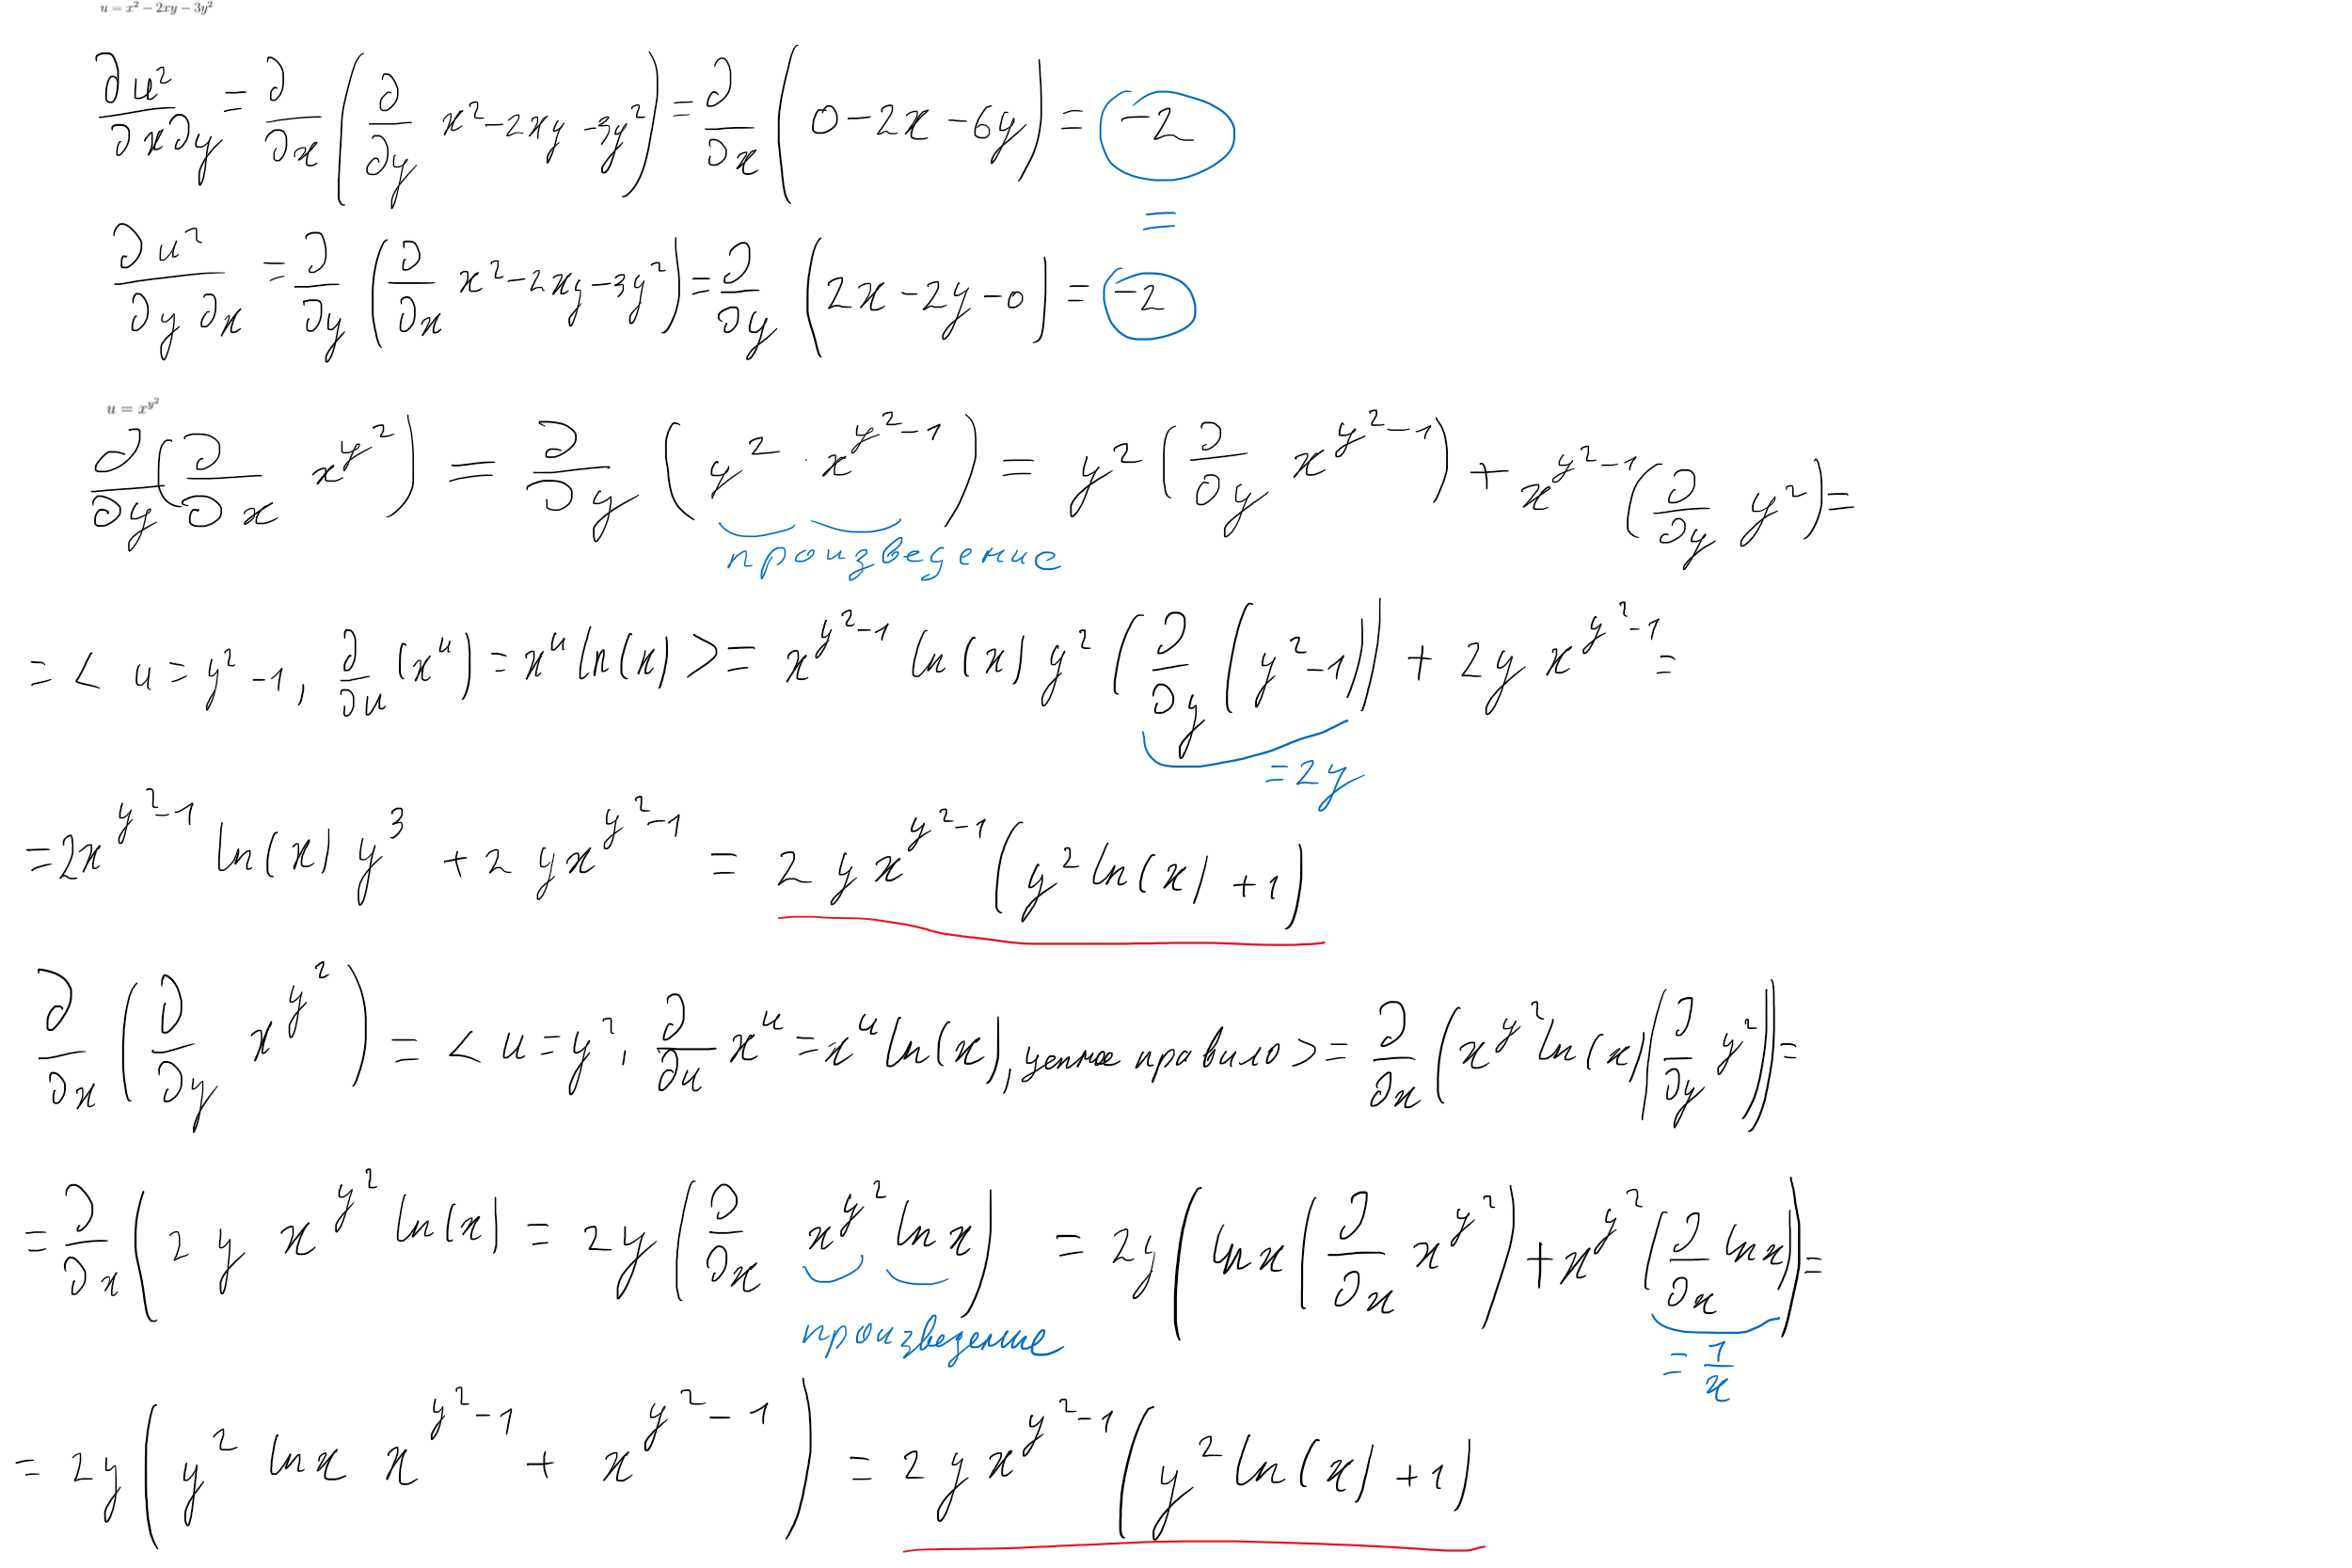
\includegraphics[width=\textwidth]{img/03.png}


\end{enumerate}

\ 

\item Найдите указанные производные
\begin{enumerate}
\item $\frac{\partial^3 u}{\partial x^2 \partial y}$, если $u = x\ln(xy)$.


\textbf{Решение:}\\
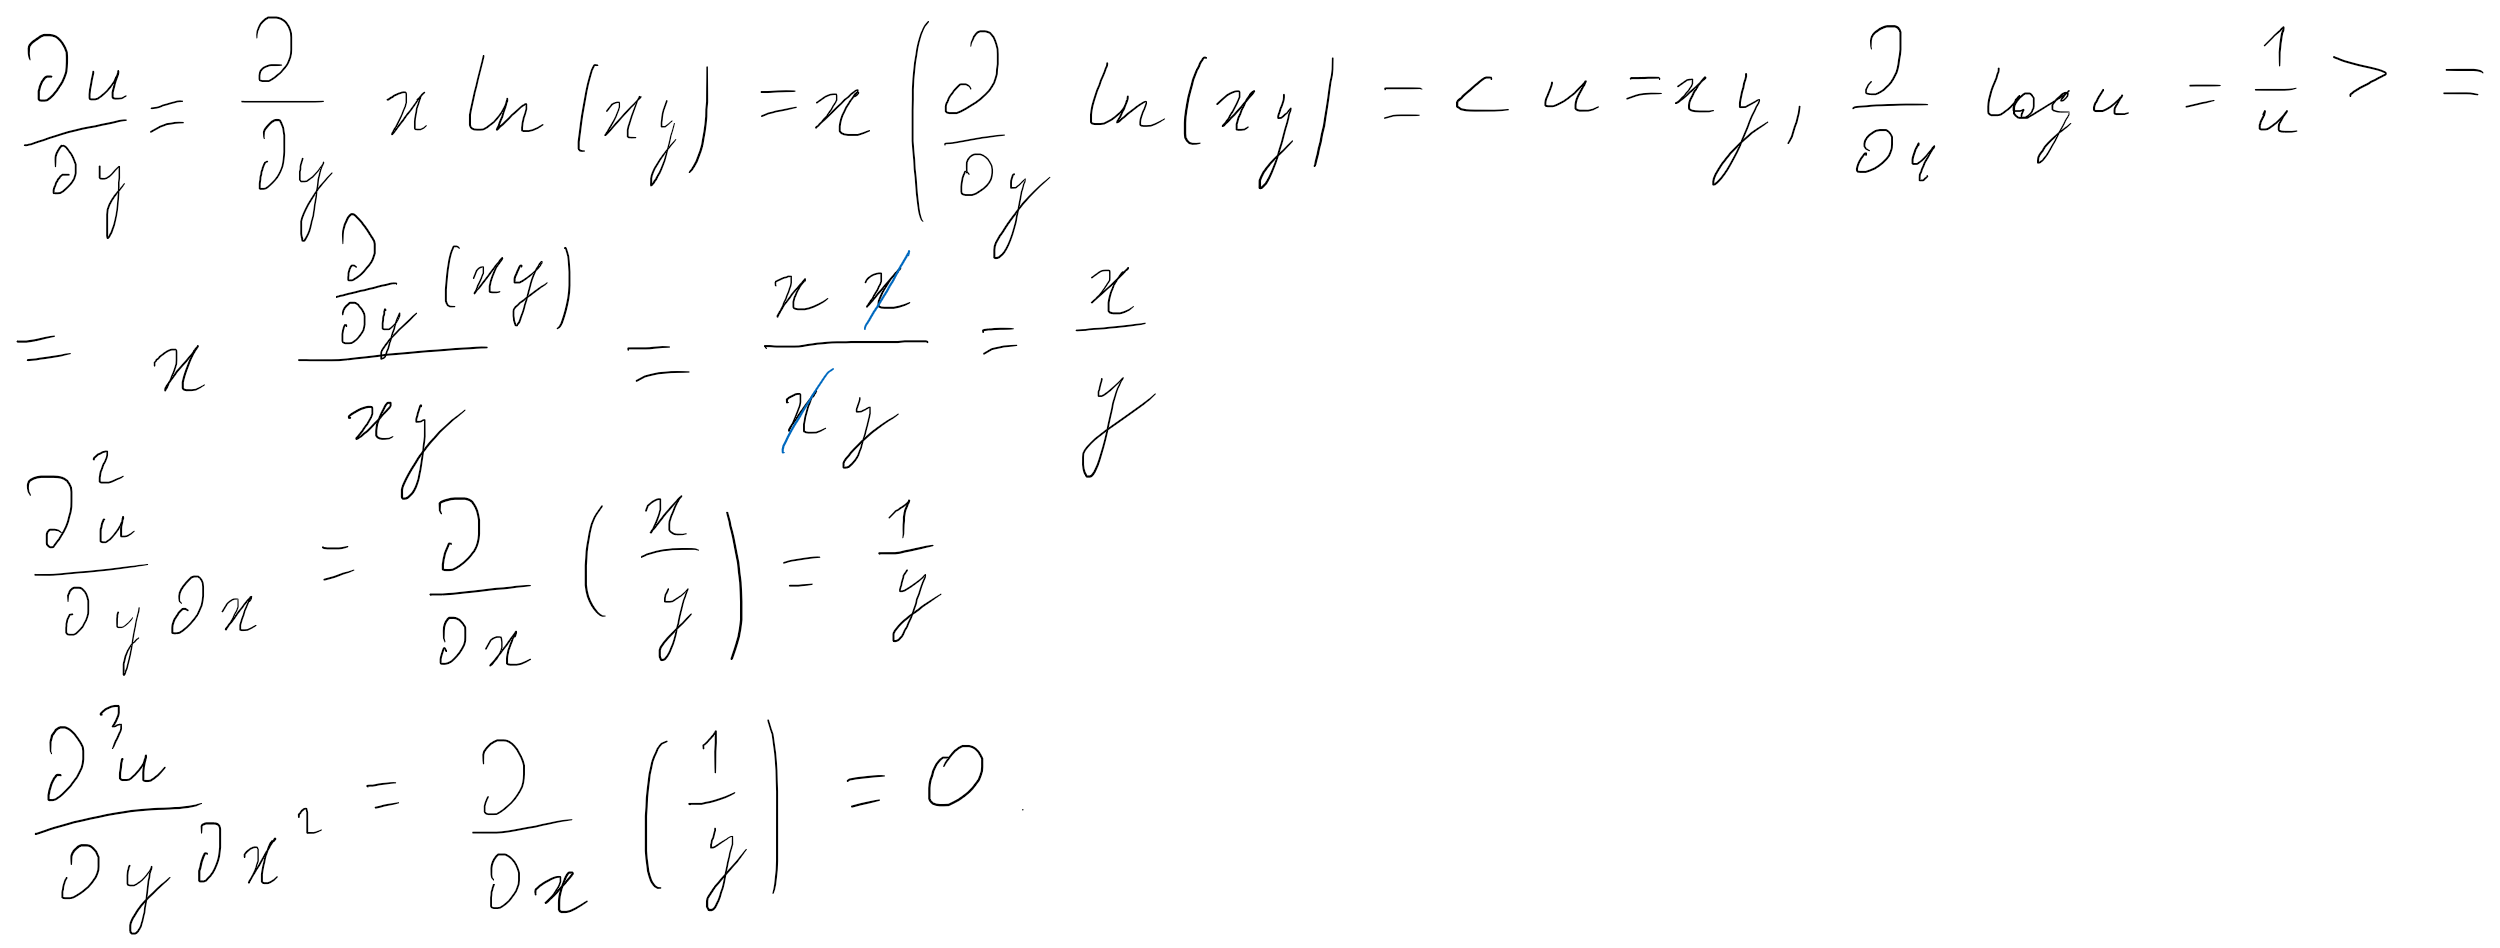
\includegraphics[width=\textwidth]{img/041.png}

\textbf{Ответ: $0$}

\item $\frac{\partial^6 u}{\partial x^3\partial y^3}$, если $u = x^3 \sin y + y^3 \sin x$.

\textbf{Решение:}\\
$\frac{\partial u}{\partial x} = 3x^2 \sin y + y^3 \cos x$


$\frac{\partial^2 u}{\partial x^2} = 6x \sin y - y^3 \sin x$


$\frac{\partial^3 u}{\partial x^3} = 6 \sin y - y^3 \cos x$


$\frac{\partial^4 u}{\partial x^3\partial y} = 6 \cos y - 3y^2 \cos x$


$\frac{\partial^5 u}{\partial x^3\partial y^2} = -6 \sin y - 6y \cos x$


$\frac{\partial^6 u}{\partial x^3\partial y^3} = -6 \cos y - 6 \cos x$

\textbf{Ответ: $-6 \cos y - 6 \cos x$}\\


\item $\frac{\partial^2 u}{\partial x\partial y}$, если $u = f(x, xy, xyz)$, где $f(y_1,y_2,y_3)=y_1+\ln(y_2y_3)-y_1y_2y_3$.


Указание: можно пользоваться тем, что частные производные можно в любом порядке применять.
\ 

\textbf{Решение:}\\
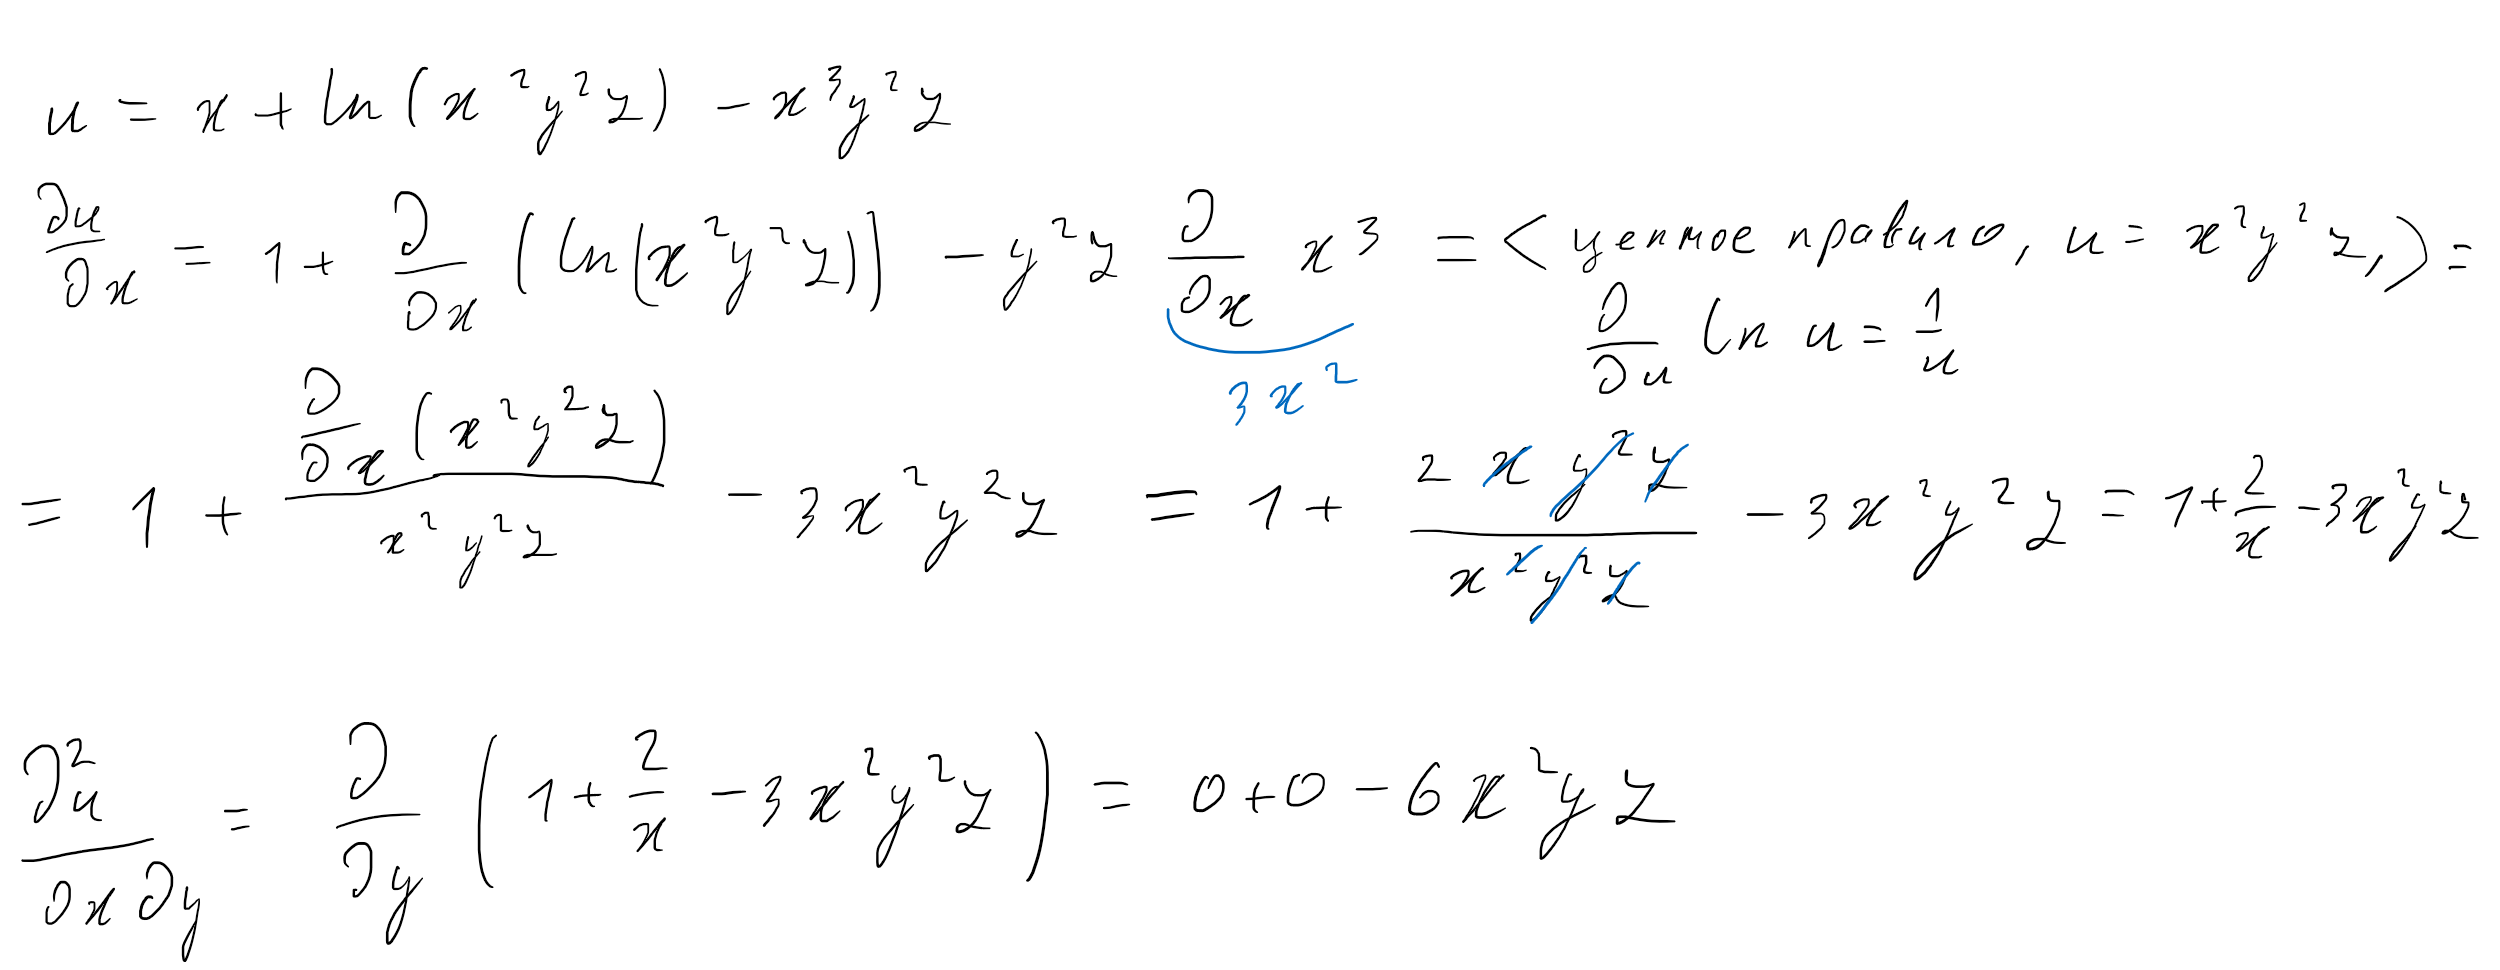
\includegraphics[width=\textwidth]{img/043.png}

\textbf{Ответ: $-6x^2yz$}


\ 
\end{enumerate}

\ 

\item Определите угол между градиентами функции $u = x^2 + y^2 - z^2$ в точках

$A = (\varepsilon , 0, 0)$ и $B = (0, \varepsilon, 0)$.


Указание: угол между векторами $v$ и $u$ можно вычислить через скалярное произведение: $$\cos\varphi=\frac{(u,v)}{|u|\cdot|v|}.$$
\textbf{Решение:}\\

Частные производные по каждой переменной x, y, z простые, весь градиент в точке будет выглядеть:

$${grad}_au = (2x(a), 2y(a), -2z(a))$$

Посчитаем значение в точках  А и В.
$${grad}_Au = (2\varepsilon, 0, 0)$$
$${grad}_Bu = (0,2\varepsilon,  0)$$

$$({grad}_Au,{grad}_Bu) = 0*2\varepsilon+2\varepsilon*0+0=0$$
$$|{grad}_Au| =|{grad}_Bu|= 2\varepsilon$$


$$\cos\varphi=\frac{0}{2\varepsilon\cdot2\varepsilon}=0$$

$\varphi=90^{\circ}$


\textbf{Ответ: Угол между градиентами $90^{\circ}$}

\item Исследовать на экстремумы следующие функции:
\begin{enumerate}
\item $f(x,y) = xy + \frac{50}{x} + \frac{20}{y}$ ($x > 0$, $y>0$).

\textbf{Решение:}\\
Выпишем градиент и матрицу Гессе
$${grad}_af = (y-\frac{50}{x^2}, x-\frac{20}{y^2})$$


$$H_a(f) = \begin{pmatrix}
\frac{100}{x^3}(a)  &  1  \\
 1 & \frac{40}{y^3}(a) 
\end{pmatrix}$$

Потенциальные экстремумы - точки, где ${grad}_af = 0$

$$\begin{cases} y-\frac{50}{x^2}=0 \\ x-\frac{20}{y^2}=0\end{cases} \Rightarrow \begin{cases} y=\frac{50}{x^2} \\ x-\frac{20}{(\frac{50}{x^2})^2}=0\end{cases}\Rightarrow   \begin{cases} y=\frac{50}{x^2} \\ x-\frac{x^4}{125}=0\end{cases}\Rightarrow   \begin{cases} y=2 \\ x=5\end{cases}$$

Рассмотрим $H_a(f)$ в точке $a=(5,2)$
$$H_a(f) = \begin{pmatrix}
\frac{4}{5}  &  1  \\
 1 & 5 
\end{pmatrix}$$
$\Delta_1 = 4/5 > 0; \Delta_2 = 4/5*5-1*1 = 3>0 \Rightarrow$ $H_a(f)$ положительно определена и точка $(5,2)$ - глобальный минимум (так как это локальный минимум и на больших значениях x, y функция положительная и стремится к $\infty$.

\item $f(x,y,z)=-x^2-5y^2-3z^2+xy-2xz+2yz+11x+2y+18z+10$.

Выпишем градиент и матрицу Гессе
$${grad}_af = (-2x+y-2z+11, x-10y+2z+2, -2x+2y-6z+18)$$


$$H_a(f) = \begin{pmatrix}
-2  &  1 &-2  \\
1  &  -10 &2  \\
 -2 & 2 &-6 
\end{pmatrix}$$

Потенциальные экстремумы - точки, где ${grad}_af = 0$
$$\begin{cases} -2x+y-2z=-11 \\ x-10y+2z=-2\\ -2x+2y-6z=-18\end{cases} \Rightarrow \begin{cases} -2x+y-2z=-11 \\ -19/2y+z=-15/2\\ -2x+2y-6z=-18\end{cases} \Rightarrow\begin{cases} -2x+y-2z=-11 \\ -19y+2z=-15\\ -2x+2y-6z=-18\end{cases} \Rightarrow$$
$$\begin{cases} -2x+y-2z=-11 \\ -19y+2z=-15\\ y-4z=-7\end{cases} \Rightarrow \begin{cases} -2x+y-2z=-11 \\ -19y+2z=-15\\ -74/19z=-148/19\end{cases} \Rightarrow\begin{cases} -2x+y-2z=-11 \\ -19y+2z=-15\\ z=2\end{cases} \Rightarrow$$
$$\begin{cases} -2x+y-2z=-11 \\ -19y=-19\\ z=2\end{cases} \Rightarrow\begin{cases} -2x+y-2z=-11 \\ y=1\\ z=2\end{cases} \Rightarrow\begin{cases} x=4 \\ y=1\\ z=2\end{cases}$$

Рассмотрим $H_a(f)$ в точке $a=(4,1,2)$

$\Delta_1 = -2 < 0; \Delta_2 = 20-1 = 19>0 ;\Delta_3 = -2*-10*-6+1*2*-2-2*1*2+2*-10*-2-1*1*-6+2*2*2=-74<0\Rightarrow$ $H_a(f)$ отрицательна определена и точка $(4,1,2)$ - глобальный максимум (так как это локальный максимум и на больших значениях x, y, z функция отрицательна и стремится к $-\infty$.
\end{enumerate}
\end{enumerate}
\end{document}